\documentclass[12pt]{article}
\usepackage[utf8]{inputenc}
\usepackage[russian]{babel}
\usepackage{graphicx}
\title{План работы}
\date{}
\author{}

\begin{document}

\maketitle
\section{Конечно-элементные вычисления.}
\subsection{Обзор конечных элементов для стационарного уравнения Стокса.}
В этом разделе мы сравниваем решения уравнений Стокса полученные с помощью различных конечных элементов.
Стационарные уравнения Стокса описывают устоявшееся несжимаемое течение в области $\Omega$ с границей $\delta\Omega$
\begin{equation}
-\Delta u + \nabla p = f \quad x \in \Omega,
\end{equation}
\begin{equation}
\nabla\cdot u = 0 \quad x \in \Omega,
\end{equation}
\begin{equation} \label{eq:stokes-boundary}
u = g \quad x \in \delta\Omega,
\end{equation}
где $u$ - поле скоростей, $p$ - поле давления и $f$ - источник. Для численного вычисления данной задачи, преобразуем ее в вариационную формулировку
\begin{equation}
a(u,v)-b(v,p)=(f,v) \quad \forall v \in V,
\end{equation}
\begin{equation}
b(u,q)=0 \quad \forall q \in \Pi,
\end{equation}
где 
\begin{equation}
a(u,v)=\int_\Omega \nabla v \cdot \nabla v \, dx,
\end{equation}
\begin{equation}
b(v,q)=\int_\Omega (\nabla \cdot v) q \, dx,
\end{equation}
\begin{equation}
(f,v)=\int_\Omega f \cdot v \, dx.
\end{equation}

Рассматриваемые наборы конечных элементов, удовлетворяющие условию Ладыженская-Бабушка-Бреззи (LBB).

Набор Тейлор-Худа.
Состоит из непрерывных элементов Лагранжа с порядком $q \geq 2$ для поля скоростей, и непрерывных элементов Лагранжа с порядком $q - 1$ для поля давления.

Набор Крузе-Равиарта.
Элемент использует интегральные моменты над ячейками границ как базис для скорости с порядком $1$, и разрывное пространство давления с порядком на $0$ меньше.

Набор CD.
Название это первые буквы от выражений continious velocity и discontinious pressure.
Для поля скоростей используется неразрывный элемент Лагранжа с порядком $q \geq 2$, для поля давления используется разрывный элемент Лагранжа с порядком $q-2$. 

Тестовой задачей является двумерное течение в каверне с подвижной верхней границей. То есть, граничное условие (\ref{eq:stokes-boundary}) переписываем в следующем виде:
\begin{equation}
u = (1, 0) \quad \partial\Omega_{t},
$$$$
u = (0, 0) \quad \partial\Omega_{w},
\end{equation}

где $\partial\Omega_{t}$ - верхняя стенка, $\partial\Omega_{w}$ - обе боковые и нижняя стенка. В постановке будем считать что две верхние угловые точки принадлежат неподвижной области $\partial\Omega_{w}$. Область представляет собой единичный квадрат, и скорость движения по $x$ верхней границы тоже $1$. Расчет проводится в безразмерных величинах, хотя можно считать сторону квадрата 1 м, и скорость стенки 1 м/с.

\begin{figure}
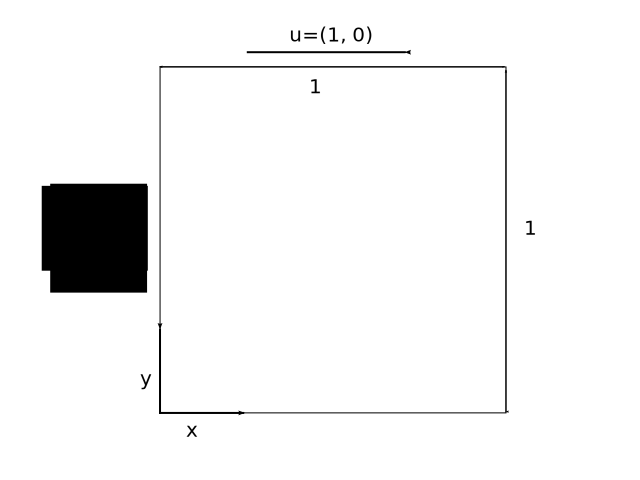
\includegraphics[scale=0.5]{stokes-test/cavity}
\caption{Тестовая область с подвижной верхней границей.}
\label{fg:cavity}
\end{figure}

Написал программу на питоне на фениксе.

Так как область квадратная, то параметром размерности задачи выбираем количество отрезков на ребре $h$. Проводились расчеты для сетки размером $h=20, 40, 80, 100$. 


Вывод графики через paraview.


Вывод графики через gnuplot.

Набор элементов Крузе-Равиарта обладает наименьшим временем решения (рис. \ref{fg:time}).
Очевидно из-за первого порядка элемента для скорости.


TODO:
- постановка задачи
    - уравнения
    - свойство уравнения
    - конечно-элементная аппроксимация
    - список выбранных элементов
        - описание элемента
        - картинка элемента? (не надо)
- решение
    - размер сетки
    - выбор элемента
        - что будет если выбрать плохой элемент
        - взять элементы на несколько порядков выше
    - "точное" решение это большее кол-во ячеек
        - надо по-тихой увеличивать кол-во ячеек и брать некую норму
        - норма должна по идее сходиться
    - приведение давления
    - сравниваем меньшее кол-во ячеек с "точным" решением
    - строим функцию тока
        - объяснение смысла функции тока
        - выбрать некий разрез для функции тока
- результаты
    - выводы
        - скорость точности элементов для функции тока
        - скорость точности элементов для скорости компоненты X
        - скорость точности элементов давления
	- график времени
	- график давления для хорошей сетки
	- график скорости для хорошей сетки
	- график функции тока для хорошей сетки
	- график изменения точности функции тока для каждого элемента
	
	


\begin{figure}
\begin{center}
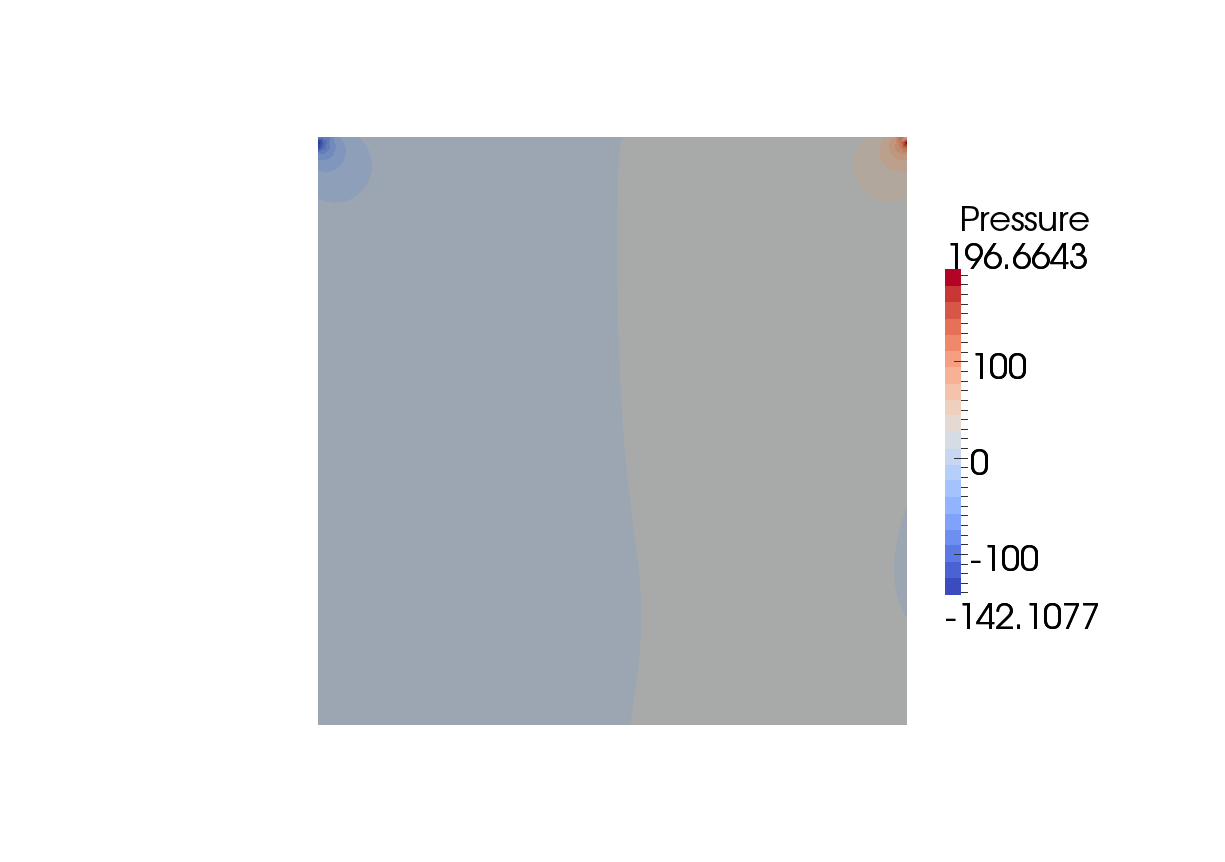
\includegraphics[scale=0.4]{stokes-test/pressure}
\caption{Поле давления.}
\label{fg:pressure}
\end{center}
\end{figure}

\begin{figure}
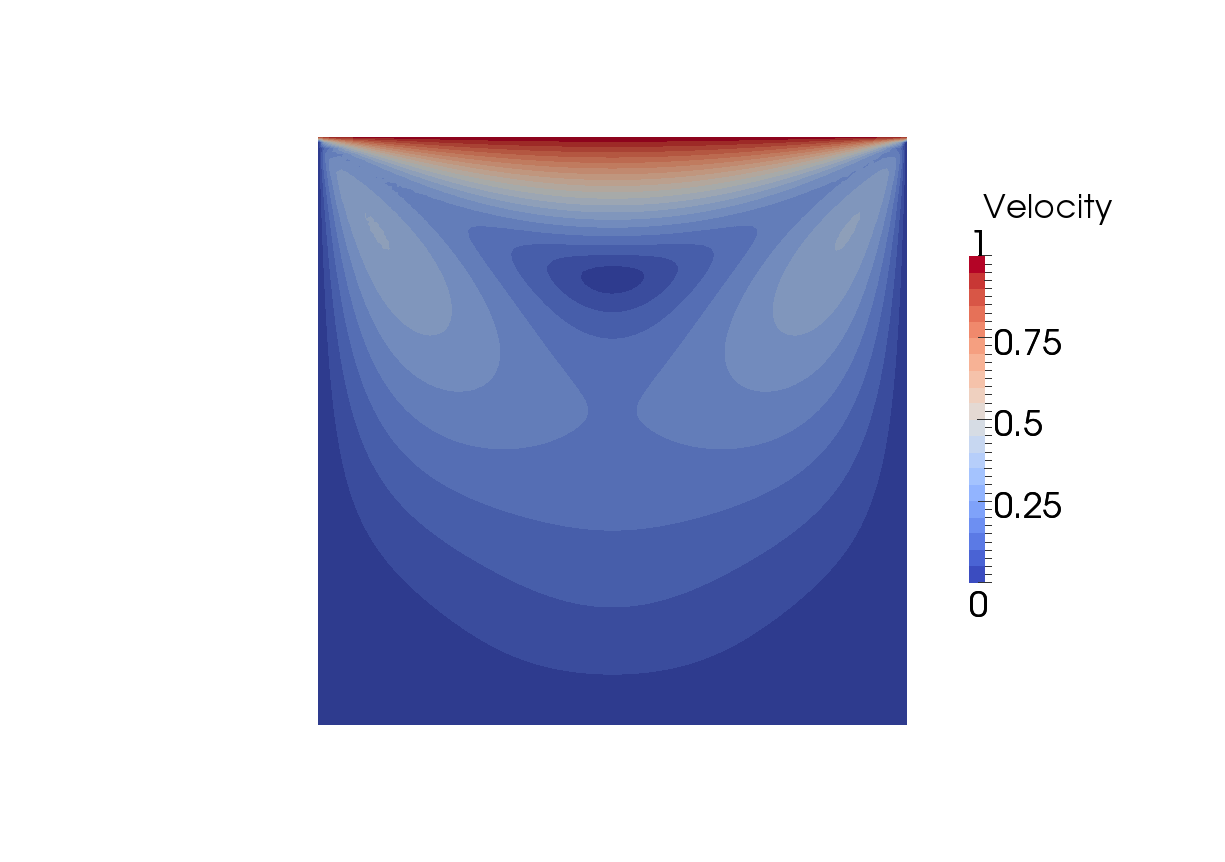
\includegraphics[scale=0.1]{stokes-test/velocity}
\caption{Поле скоростей.}
\label{fg:velocity}
\end{figure}

\begin{center}
  \begin{figure}
    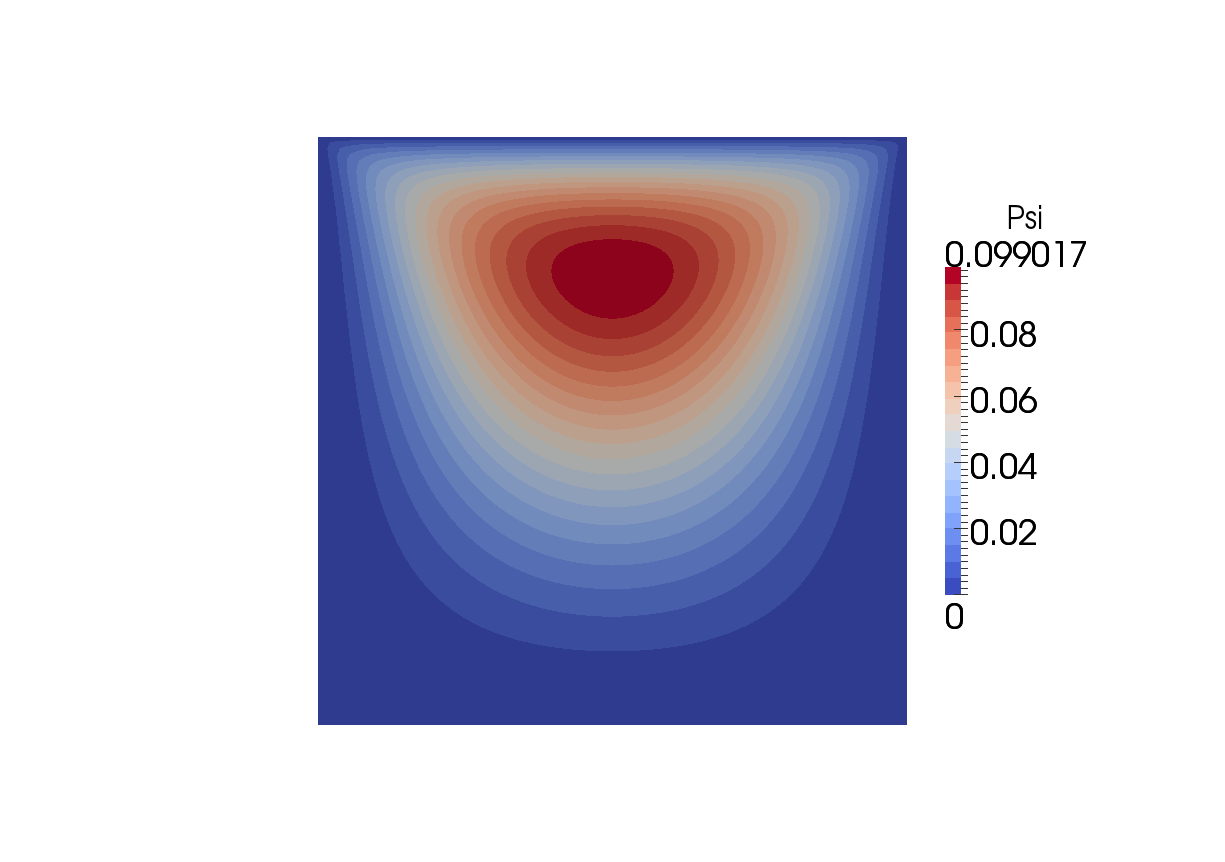
\includegraphics[scale=0.4]{stokes-test/psi}
    \caption{Поле функции тока.}
    \label{fg:psi}
  \end{figure}
\end{center}

\begin{figure}
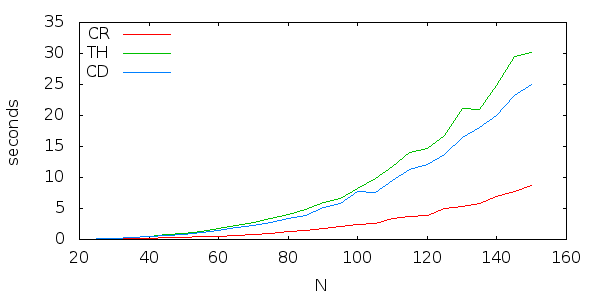
\includegraphics[scale=0.1]{stokes-test/time}
\caption{Зависимость времени решения от кол-ва ячеек.}
\label{fg:time}
\end{figure}

\subsection{Схемы расщепления.}
\subsection{Аппроксимация конвективного слагаемого для уравнения Навье-Стокса.}

\section{Осесимметричная задача моделирования несущей конструкции.}
\subsection{}

\section{Трехмерное моделирование несущей конструкции.}
\subsection{}

\end{document}